\documentclass{standalone}
\usepackage{tikz}
\begin{document}
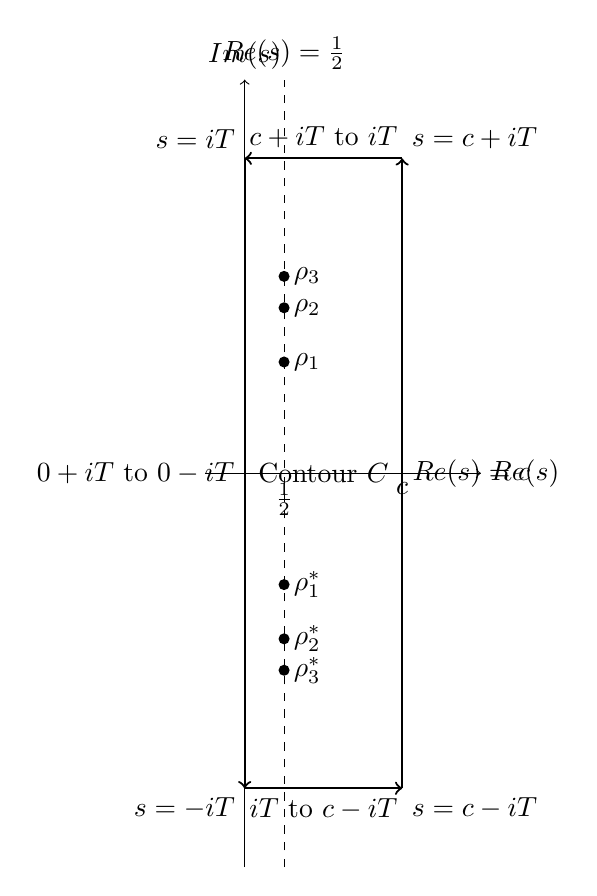
\begin{tikzpicture}
% Axes
\draw[->] (-0.5,0) -- (3,0) node[right] {$\text{Re}(s)$};
\draw[->] (0,-5) -- (0,5) node[above] {$\text{Im}(s)$};

% Contour path (counterclockwise)
% Vertical line at Re(s) = c (c = 2), from -T to T
\draw[thick,->] (2,-4) -- (2,4) node[midway,right] {$\text{Re}(s) = c$};
% Top segment from (c, T) to (0, T)
\draw[thick,->] (2,4) -- (0,4) node[midway,above] {$c + iT$ to $iT$};
% Left vertical segment at Re(s) = 0, from T to -T
\draw[thick,->] (0,4) -- (0,-4) node[midway,left] {$0 + iT$ to $0 - iT$};
% Bottom segment from (0, -T) to (c, -T)
\draw[thick,->] (0,-4) -- (2,-4) node[midway,below] {$iT$ to $c - iT$};

% Poles along Re(s) = 1/2 at approximate RZF zeros
\foreach \y/\label in {1.4135/$\rho_1$, 2.1022/$\rho_2$, 2.5011/$\rho_3$, -1.4135/$\rho_1^*$, -2.1022/$\rho_2^*$, -2.5011/$\rho_3^*$} {
  \fill (0.5,\y) circle (2pt);
  \node[right] at (0.5,\y) {\label};
}
\draw[dashed] (0.5,-5) -- (0.5,5) node[above] {$\text{Re}(s) = \frac{1}{2}$};

% Labels for vertices
\node[below right] at (2,-4) {$s = c - iT$};
\node[above right] at (2,4) {$s = c + iT$};
\node[above left] at (0,4) {$s = iT$};
\node[below left] at (0,-4) {$s = -iT$};

% Annotation for contour direction
\node at (1,0) {Contour $C$};

% Mark Re(s) = 1/2 on the real axis
\node[below] at (0.5,0) {$\frac{1}{2}$};
\node[below] at (2,0) {$c$};
\end{tikzpicture}
\end{document}